%% ----------------------------------------------------------------
%% Results.tex
%% 333 ---------------------------------------------------------------- 
\chapter{Results \& Discussion} \label{Chapter: Results}

% Parameters are defined in Results (not in Methods)

% Report is a presentation of the final results, not the whole process.

% Draw inferences from proofs

% Check that your paper is focused. Choose the point of the paper and its key conclusion before you begin writing, stick to your choices, and write the paper so that the reader gets the point already in the abstract and in the introduction. Leave  out results that are not required for supporting the key conclusion, or safely tuck them away in the supplementary information document. When editing, if you feel that your paper loses its focus at some point, take a step back and do a major rewrite.

% Check that there is a clear question and a clear answer—it is all too common to focus on your results and what you have done, instead of stating and then solving a problem. Your results are meaningful only if they solve a meaningful problem. Remember that your paper is neither an account of your work nor a lab diary; it should be a story of an important problem and its solution. Emphasise the problem, both in the Introduction where it should really stand out, and in the Results section and the Discussion. Make it clear to the reader how each result contributes to solving the problem, and what the implications of solving the problem are.

%\begin{enumerate}
%\item What did I find?
%\item Let me describe the best bits
%\item Here is my analysis and proof of it
%\item Here's my conclusion(s) about it
%\end{enumerate}

I have trained the network described in section \ref{sect:network} for 400 epochs with the same parameters as the ones used by \cite{Jurtz2017}; i.e., gradient clipping at 20, regularization term $\lambda=10^{-3}$, and training-validation split at the 5278th sequence. The resulting network reaches an accuracy of 67.7\% on the test set, which is not far from the 71\% of the state-of-the-art (see section \ref{sect:HoF}).
I believe that the techniques of analysis here presented and the conclusions withdrawn from them can be transferred to current state-of-the-art methods without losing validity.

\section{Outlier analysis} \label{sect:outliers}

In order to analyse the performance space a bit better, the average accuracy per sequence has been calculated and it has been plotted in Figure \ref{fig:per_seq_acc} with respect to the sequence length. The distribution exhibits the typical funnel shape that one could expect from processes with random variables forming groups of different sizes: the bigger the groups, the smaller the variance. The funnel ceases to shrink at length about 400, so it would be particularly interesting to understand why the network is classifying worse (60\% and below) some of the sequences above that length.

% CHeck alpha-helix size
If we observe the colour scheme of the figure, we can understand right away that sequences rich in $\alpha$-helix are generally better predicted than $\beta$-sheets and coils. An explanation could be that while $\alpha$-helix sizes are up to CHECK NUMBER, which is inside the window size, $\beta$-sheets interact with amino-aids further away in the sequence, which is not possible to be captured with the window of the network, of lateral size of 9.

\begin{figure}
\centering
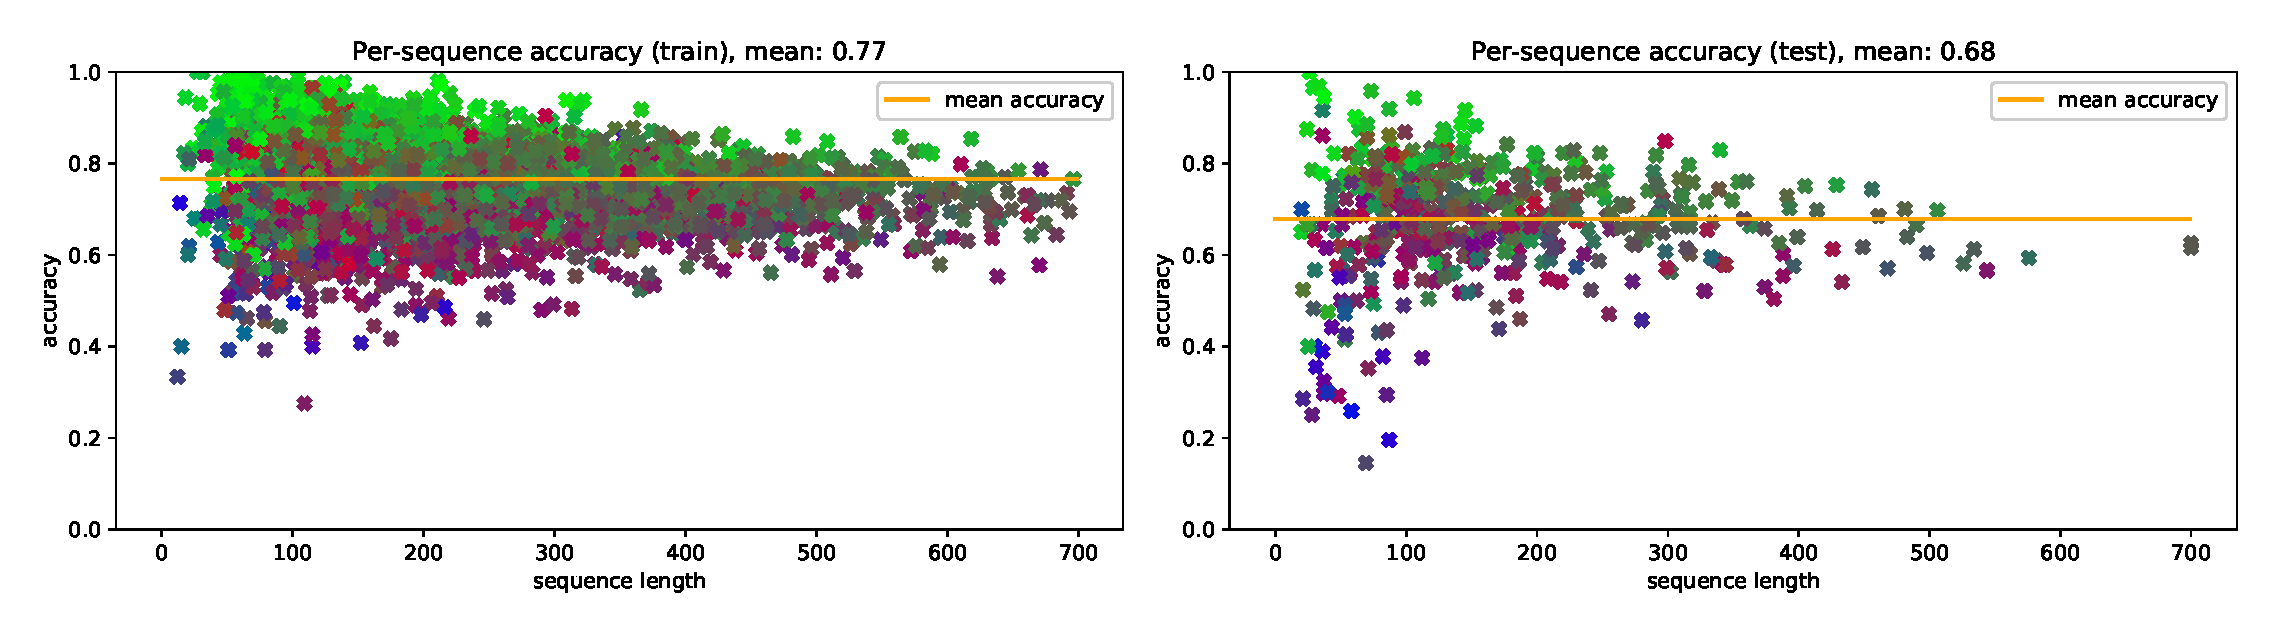
\includegraphics[width=1\linewidth]{Figures/per_seq_acc}
\caption{\textit{The mean accuracy per sequence by sequence length.} The 5504 sequences of the training set are shown on the left and the 514 of the test set on the right. Each point represents a single protein, and its colour corresponds to the amount of $\beta$-sheets (red), $\alpha$-helices (green), and coils (blue) it has. A purple point, for instance, would predominantly have $\beta$-sheets and coils.}
\label{fig:per_seq_acc}
\end{figure}
% EXtra: include the same graph but colour the high-appearing classes and the low appearing classes differently (RB)

\section{Feature visualization}

	\subsection{First layer filters}
	
	\subsection*{Saliency maps on layers?}


\section{Saliency maps on inputs}

Before going through the analysis, it is worth commenting that the saliency map outputs have many dimensions, since each position at each sequence has a saliency map with shape 8x42x19, corresponding to the 8 classes (outputs), the 42 inputs and and the total window size of 19. The results can be shown in multiple ways, depending on which dimensions are preserved and which are aggregated. 

%Talk about dimensions: saliency value, class, sequences, positions, window, amino-acids, aa/pssm (7 dimensions). From now on, individual saliency maps will refer to the saliency map of one sequence-position

\subsubsection*{Analysis on amino-acids and \textit{pssm}}
When looking at typical secondary-structure prediction algorithm, there is one point that may raise some suspicion: the inclusion of half of the inputs as one-hot encoded (amino-acids) and the other half as dense vectors (\textit{pssm}). One could thing that this discrepancy may strongly favour the information coming from the dense part, since the weights associated to it will learn much faster in a typical gradient descent learning schema.

Saliency maps can be used to prove whether this hypothesis is right by inspecting which of the input groups is being most decisive in the classification process. For doing so, each saliency map is divided into two groups of $8x21x19$, and all the values inside each group are added up to a single \textbf{saliency score}. Thus, each position of each sequence will have two scores, one for the amino-acids and one for the \textit{pssm}, and its comparison will give us which part of the inputs is more decisive. The results are shown in Figure \ref{fig:aa_pssm}, from where it can be appreciated that there are considerably more positions in which the input from \textit{pssm} was more determinant (around 1.1 millions) than the ones with more determinant amino-acid inputs (about 200 thousands). Furthermore, in most of the cases amino-acid inputs had more impact it was only by a narrow margin, with 70\% of the cases having only up to two times bigger saliency scores. On the contrary, more than 60\% of the positions with higher \textit{pssm} saliency score did this with a more than twice higher score.

\begin{figure}
\centering
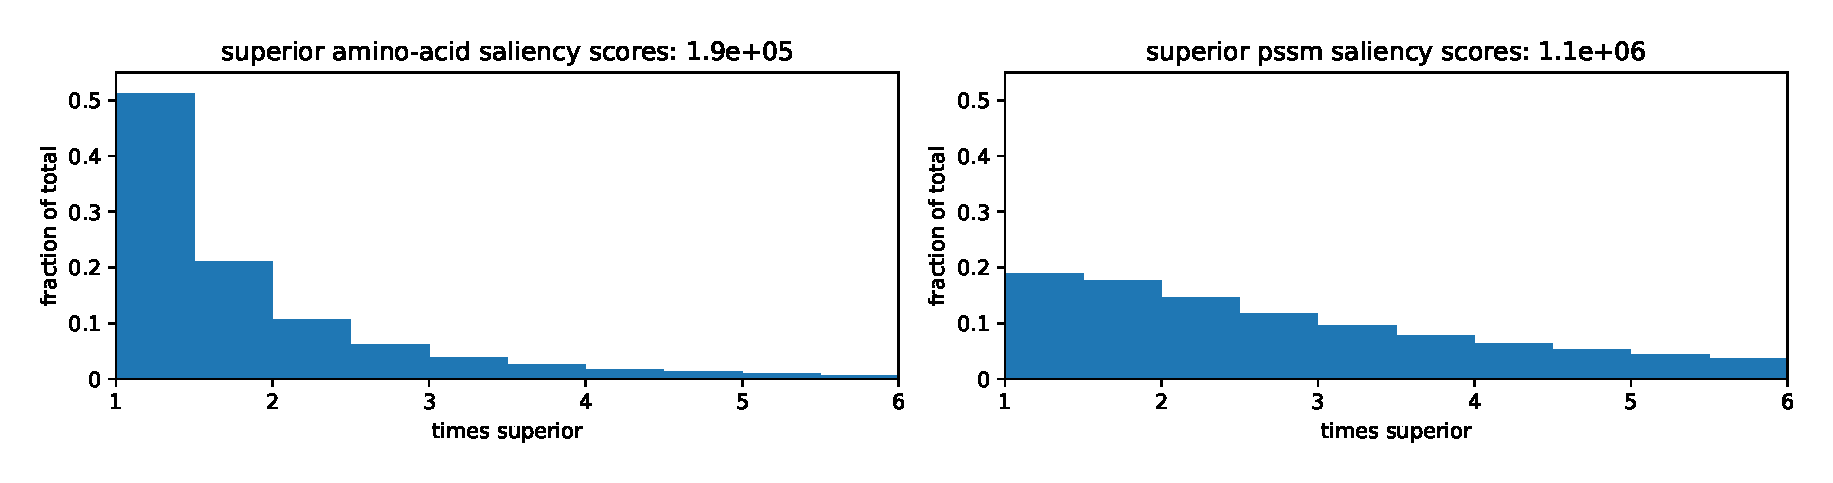
\includegraphics[width=1\linewidth]{Figures/aa_pssm}
\caption{\textit{Amino-acids versus pssm comparison.} On the left, a histogram of the positions whose amino-acid saliency score was higher than the pssm score, with the total amount in the title. The bins represent the superiority ratio, i.e. how many times bigger was the score. On the right, the analogous histogram for pssm superior scores.}
\label{fig:aa_pssm}
\end{figure}


%Options (all options could be applied either to aa or to pssm, 6 dimensions left)
	
	\subsection{Sequence-specific saliency maps}
	This section will present the sort of analysis that can be done for a specific sequence. This can be specially useful for analysing the sequences whose accuracy was remarkably lower (outliers). Each sequence has a number of saliency maps equal to its length, $l$, and they can either be inspected one by one or be overlapped through the sequence, obtaining a single 8x42x$l$ \textbf{sequence map}.
	
	% analyse per-class single sequence (sample-based) (4 dimensions left): aa-aggregated (3 dimensions) and added in the sequence position, either respecting each position (3 dimensions) or aggregating them in a heat map (2 dimensions), or aggregating the positions in a heat-map but containing the 8 classes (3 dimensions) (Colour the labels with the RGB either form Figure \ref{fig:per_seq_acc} or with the colour code from \ref{sect:sheer}).
		
	%Have the x labels including amino-acid, prediction, and real label. Colour classes with the codes mentioned in the previous paragraph. Consider marking mismatches in bold.
	
	Figure \ref{fig:sliding} shows consecutive saliency maps belonging to a single class. The patterns they present are generally preserved (note the differences in scales), just being shifted by one position on the window axis. This suggests that the algorithm is not differentiating that much between specific amino-acid positions, but rather looking for them to be in the vicinity. For this reason, we can consider that overlapping them in a single sequence map does preserve most of the information, as it is shown in Figure \ref{fig:sample_8classes}. This sort of map reveals which amino-acids of the vicinity are mostly responsible for a prediction in a particular position. For instance, the  predictions of class \textit{E} on the left side of the shown fragment have to do with the presence of amino-acids \textit{A}, \textit{V} and \textit{L}, while the failure to predict class \textit{H} on position 109 is likely related to the presence of amino-acid \textit{D} at position 110. Note that these saliency values come from the aggregation of all the 42 inputs and not only from the one-hot encoded side, which explains why positions 105 and 106 have different values in spite of having the same amino-acid (\textit{D}). For a deeper look into the whole \textit{pssm} spectrum, we would need to narrow the scope down to a single class, as it is done in Figure \ref{fig:sample_Hclass}. This figure reveals that is indeed common that the real amino-acid in the sequence is not among the most influential ones from the \textit{pssm} for making the decision. Note that the pssm values of the amino-acids not always need to have contributions of the same sign (such as \textit{P} or \textit{D} in the figure), revealing that the network is capturing something more than pure presence: location and combinations of amino-acids are also important.
	
	\begin{figure}
	\centering
	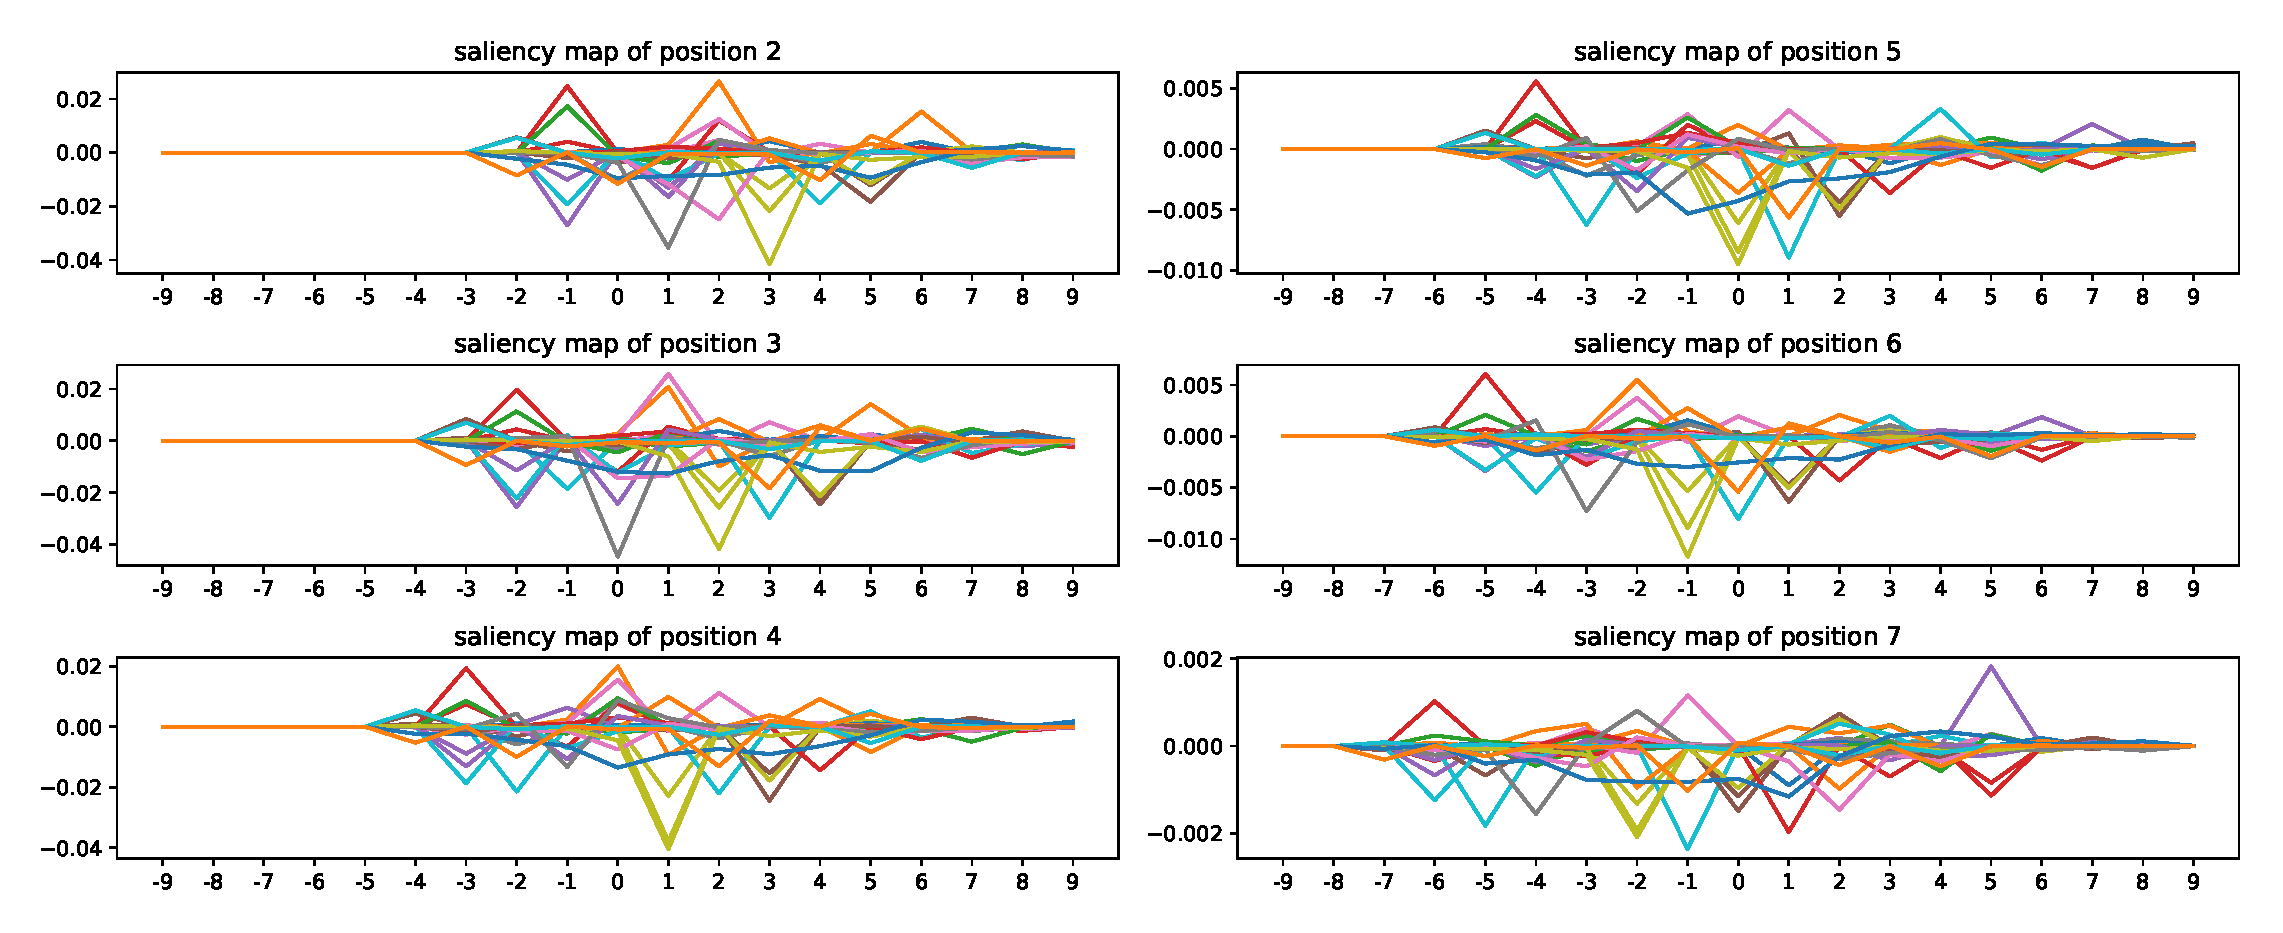
\includegraphics[width=1\linewidth]{Figures/sliding}
	\caption{\textit{Saliency maps for consecutive positions in a sequence.} In every sub-figure there are 42 lines of the 42 inputs, corresponding to their saliency values for class \textit{H}.}
	\label{fig:sliding}
	\end{figure}

	
	\begin{figure}
	\centering
	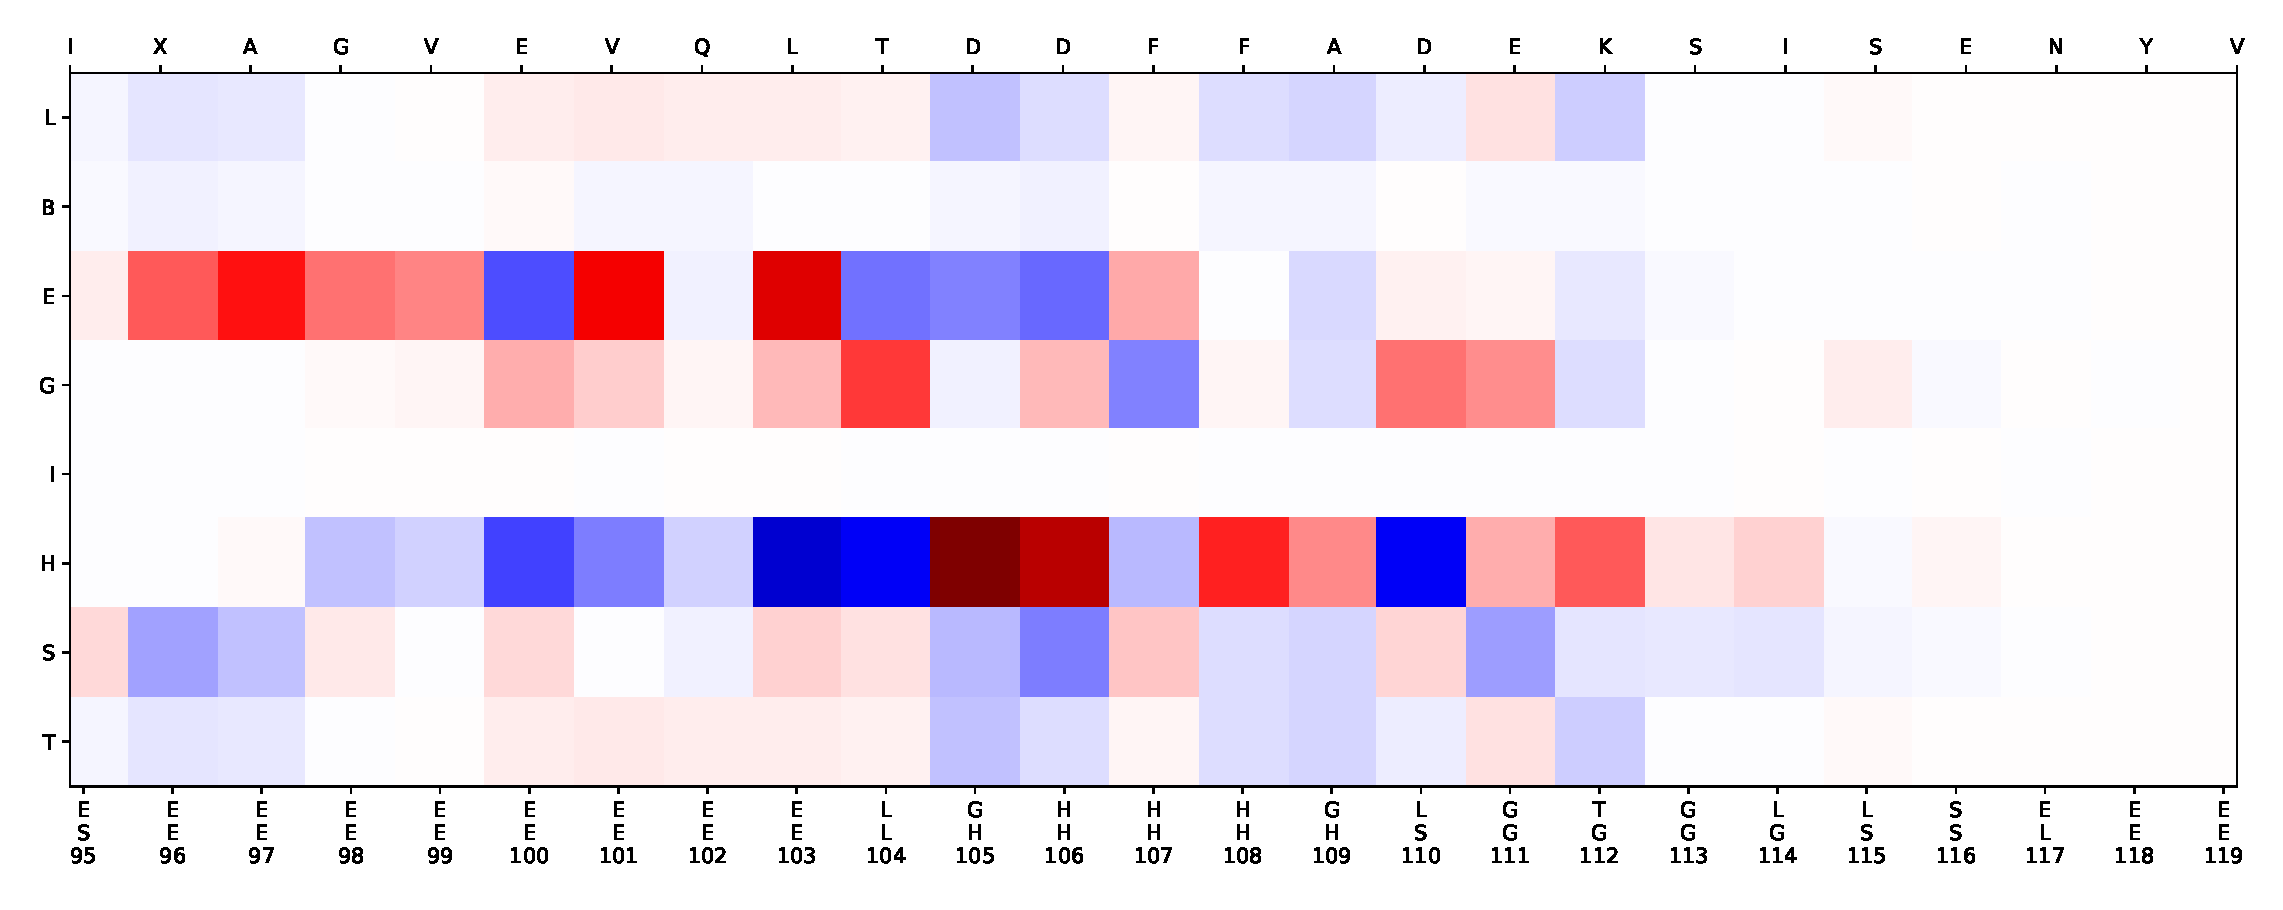
\includegraphics[width=1\linewidth]{Figures/sample_8classes}
	\caption{\textit{Fragment of a sequence map aggregated by input.} Each line corresponds to the aggregated saliency values of one of the eight output classes. The upper $x$ axis displays the amino-acids in the sequence. The labels at lower $x$ axis contains three sets of labels in this order: the predictions, the true values, and the positions in the sequence. The code of colours of the labels is the same as the lines and is set according to the class of the predictions.}
	\label{fig:sample_8classes}
	\end{figure}
	
	\begin{figure}
	\centering
	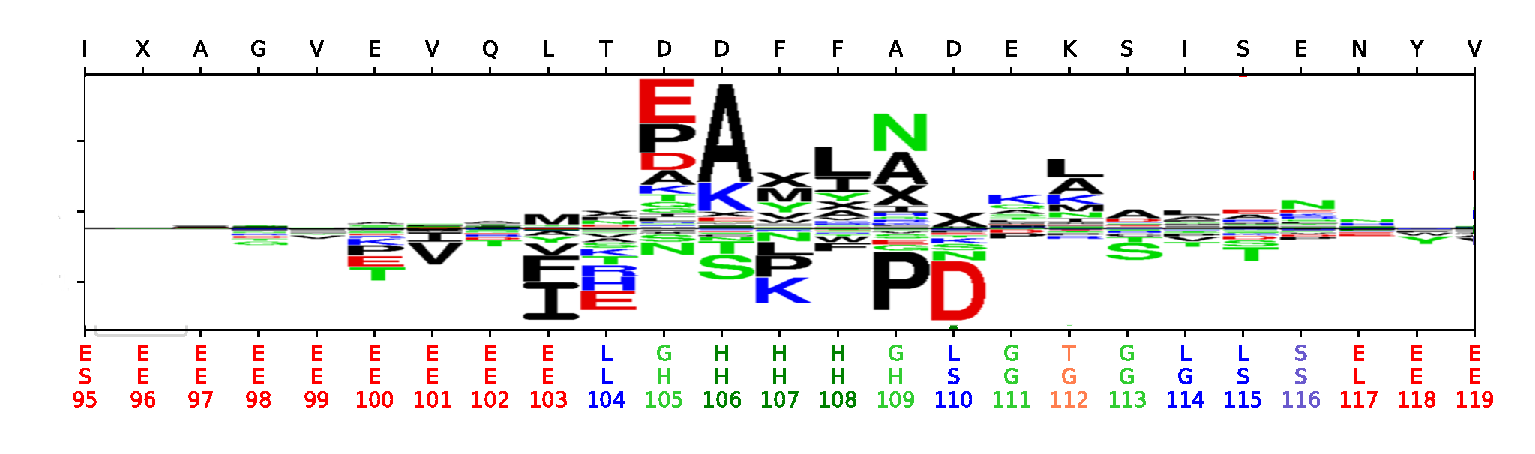
\includegraphics[width=1\linewidth]{Figures/sample_Hclass}
	\caption{\textit{Fragment of sequence map for class H.} The layout of the figure is the same as of Figure \ref{fig:sample_8classes}. The image has been generated by \textit{SeqLogo} \cite{Thomsen2012}.}
	\label{fig:sample_Hclass}
	\end{figure}

	
	% HAve as the sample one of the sequences with low accuracy and high length from \ref{sect:outliers}?

	\subsection{Class-specific saliency maps}
	Instead of looking at the saliency information along single sequences, aggregating the information from all the 1.3 millions saliency maps could give us some broader information of what the network has learned. Again, the high dimensionality of the data to explore requires us to seek for meaningful ways to aggregate and represent the data.
	
		\subsubsection*{Sheer addition} \label{sect:sheer}
		A simple way to aggregate the saliency maps would be adding them up with element-wise addition, thus composing a single saliency map of size 8x42x19. This mega-saliency map should convey rough information of the general features of the network. Since there is no a sense of ``left" or ``right" in the sequences, the aggregation should be \textit{side-invariant} and therefore an extra \textit{mirroring} operation is applied to the aggregation in order to make the aggregated saliency map symmetric along the centre of the window.
		
		To start with, Figure \ref{fig:class_agg_class} shows the aggregated saliency maps of the three main classes. There are a few details to notice here. First, higher saliency values concentrate around the centre of the window, meaning that most relevant information is located around 5 positions from the predicted one. Second, most amino-acids preserve the same sign along the window of a class, although a few exceptions also occur. Third, as it could be expected, class \textit{L} generally presents inverse patterns w.r.t. classes \textit{H} and \textit{E}. This makes sense since coils appear wherever there are no $\alpha$-helices or $\beta$-strands, they are complementary. Lastly, each class has a ``feature amino-acid" that is their best indicator, amino-acid \textit{A} for class \textit{H}, \textit{V} for \textit{E}, and \textit{P} for \textit{L}.
		
		\begin{figure}
			\centering
			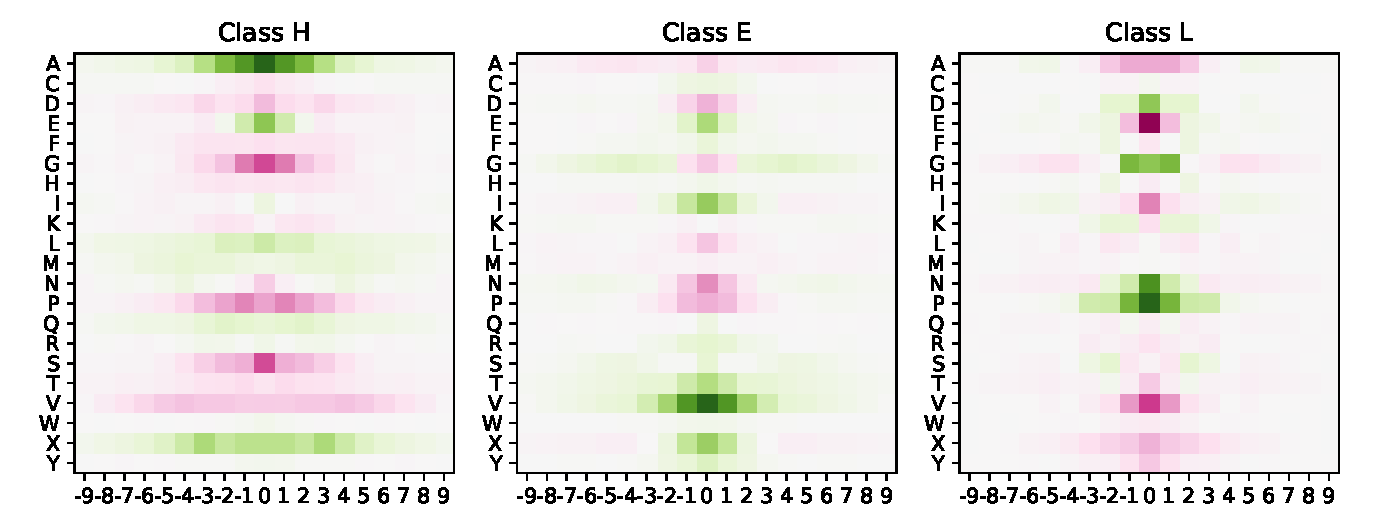
\includegraphics[width=1\linewidth]{Figures/class_agg_class}
			\caption{\textit{Per-class aggregated saliency maps of the main three classes along the window.} Only the saliency of \textit{pssm} value is shown here. Green means positive saliency values and purple means negative.}
			\label{fig:class_agg_class}
		\end{figure}
		
		Figure \ref{fig:class_agg_aa} shows the same information from the mega-saliency map but from a different perspective: it focuses on how a single amino-acid and shows how its position affects its influence on the the eight classes. As it has been discussed above, the \textit{one-hot encoded} amino-acid half of the input appears to be less significant than the \textit{pssm} half (about one fifth in this case). Both graphs show similar patterns, although it differs more for some other amino-acids (not shown). The figure shows that amino-acid \textit{G} favours $\beta$-strands on its sides and \textit{turns} and coils on its spot. 
		
		\begin{figure}
			\centering
			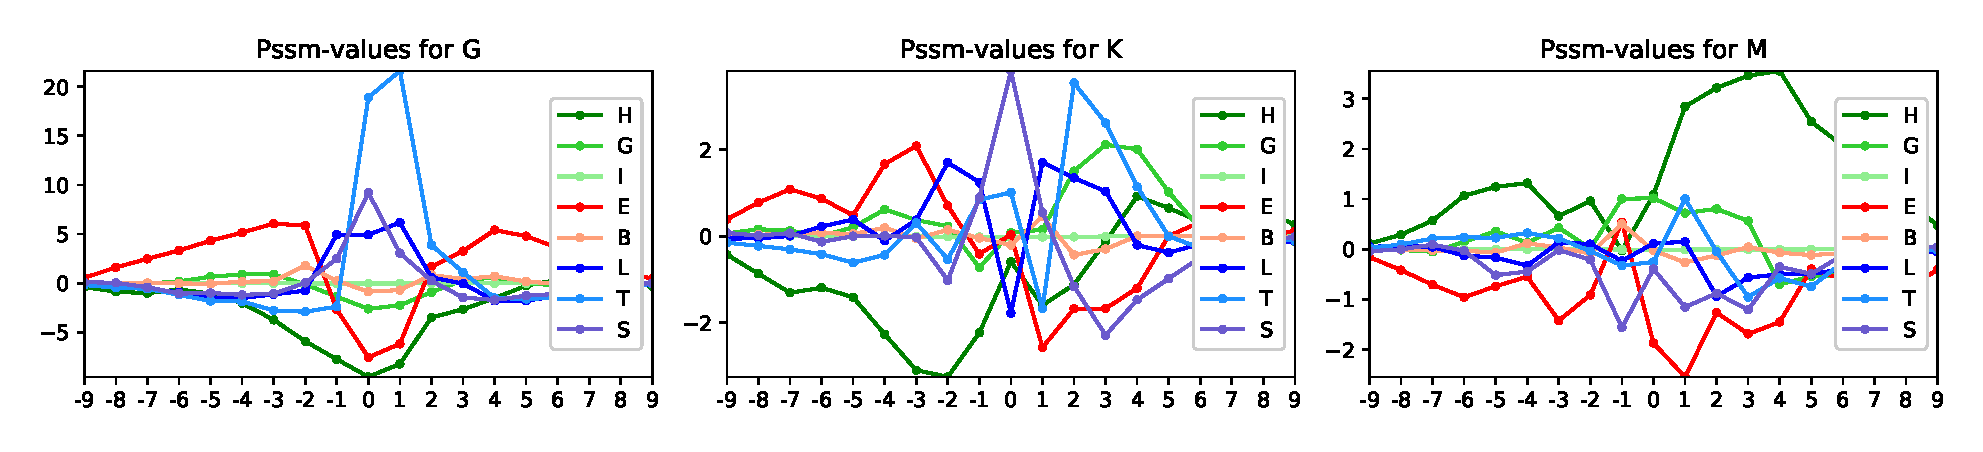
\includegraphics[width=1\linewidth]{Figures/class_agg_aa}
			\caption{\textit{Per-class aggregated saliency map of for amino-acid G along the window.} On the left the information from the \textit{one-hot encoded} part, on the right the values corresponding to the \textit{pssm} half of the input; plotted in different scales.}
			\label{fig:class_agg_aa}
		\end{figure}


		% SHould I try to compare my results with known motifs? Absolutely yes!

			\subsubsection*{Per-aminoacid and class aggregations}
			% INclude per-class aggregations (absolute value, aa aggregated) -> class profile (flatness, distribution, etc)
			% XAxis labels should be centered on 0 and going to +-9
			\begin{figure}
		\centering
		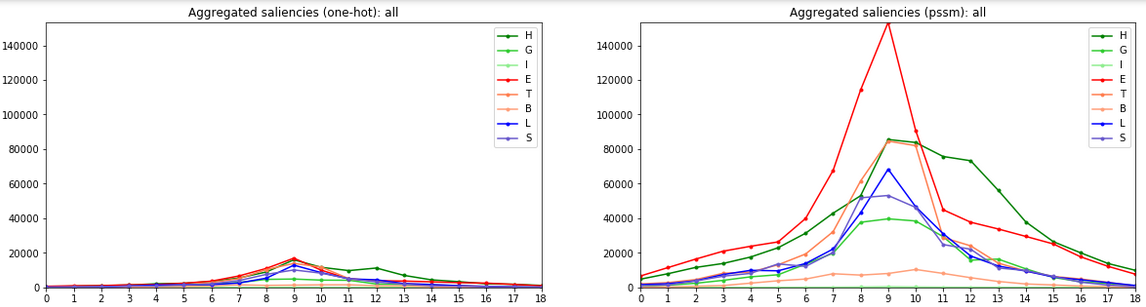
\includegraphics[width=1\linewidth]{Figures/per-class}
		\caption{}
		\label{fig:per-class}
		\end{figure}
			
			
	
		\subsubsection*{Clustering techniques}
		aggregate all individual saliency maps % SHould I try to compare my results with known motifs? Absolutely yes!
		%clustering (5 dimensions left)
		%Using the per-class window-aggregated version of individual saliency maps (4 dimensions left)
		%Cosine distance metric.
		%Show either all profiles per-cluster (3 dimensions), or aggregated profiles (2 dimensions)
		%Show t-SNE with points coloured by cluster
		
		\begin{figure}
\centering
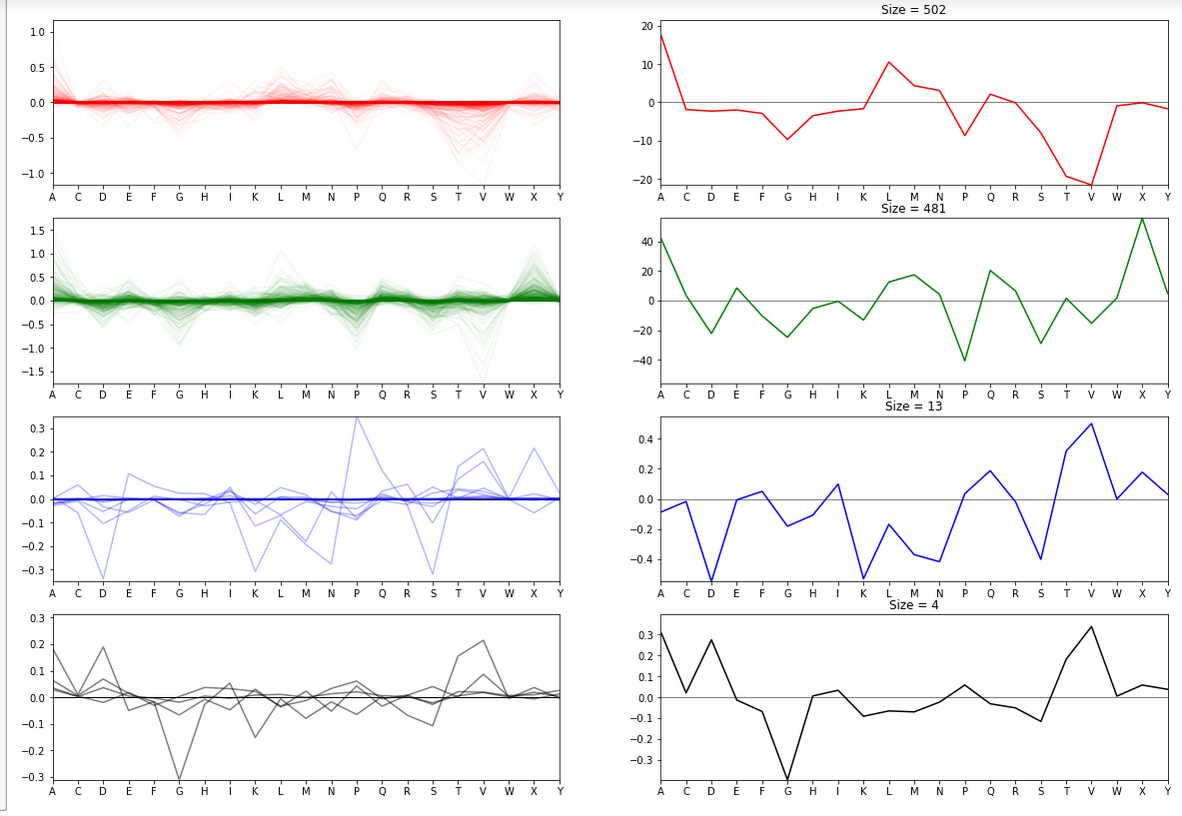
\includegraphics[width=1\linewidth]{Figures/clusters}
\caption{}
\label{fig:clusters}
\end{figure}

\begin{figure}
\centering
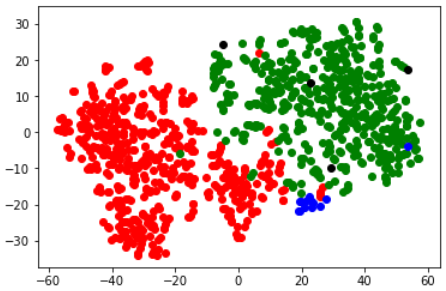
\includegraphics[width=0.7\linewidth]{tsne}
\caption{}
\label{fig:tsne}
\end{figure}

